\chapter{绪论}

\section{福斯特共振能量转移(FRET)}

\subsection{FRET原理概述}

\ifshowtext
1948年,Förster首次阐述了福斯特共振能量转移(Förster Resonance Energy Transfer,FRET)理论。FRET是指处于激发态的供体分子(Donor)通过偶极子间相互作用将一部分能量以非辐射的形式转移给邻近处于基态的受体(Acceptor)分子(供受体之间的距离R在0~10 nm)。FRET 的发生会使得供体的荧光淬灭和受体的荧光增强,其中由于发生FRET而增强受体荧光称为敏化发射荧光。FRET技术突破传统观测局限,精准解析分子间相互作用与距离。在细胞生物学微观环境里,FRET技术如同精密“分子尺”,捕捉纳米尺度生物分子动态,助力剖析分子结构与功能。因而,FRET技术在细胞生物学多领域,如细胞信号转导、蛋白质相互作用探测等广泛应用。

FRET双杂交分析是目前唯一能够在活细胞内实现生物大分子“滴定”实验的技术。蛋白质之间相互作用的化学计量比是阐明蛋白质间相互作用机制的重要参数,FRET双杂交分析通过结合受体中心的33-FRET和供体中心的E-FRET方法,能简单稳健地得到活细胞中生物复合物化学计量比和相对亲和力常数。
\begin{figure}[htbp]
    \centering
    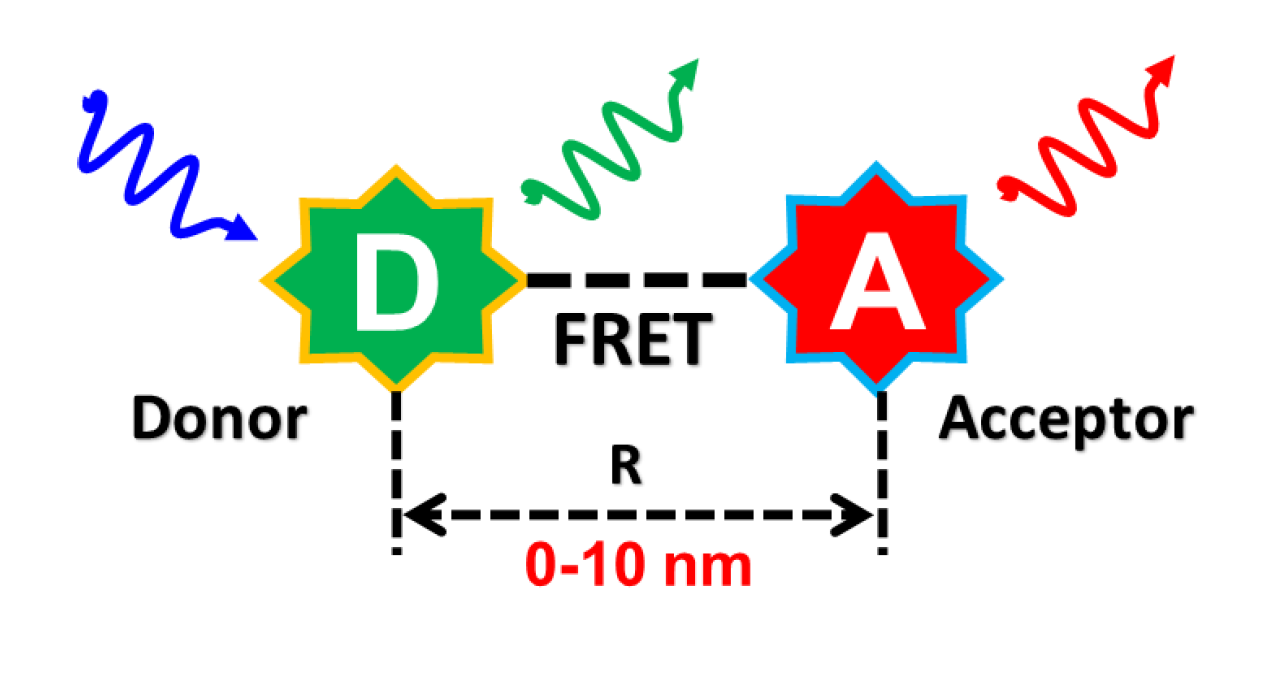
\includegraphics[width=0.5\linewidth]{../figures/1/1_FRET过程示意图.png}
    \caption{FRET过程示意图}
    \label{fig:fret}
\end{figure}

理论和实验证明,当供受体荧光分子的距离为$r$时,它们之间的能量转移速率由下式给出:
\begin{equation}
    k_T(r)=\frac{1}{\tau_D}(\frac{R_0}{r})^6, \label{eq:1-1}
\end{equation}
其中$\tau_D$是供体荧光寿命,$R_0$为Förster半径,由下式表示:
\begin{equation}
    R_0^6=8.79\times{10^{-5}}(n^{-4}Q_DJ(\lambda)\kappa^2),
\end{equation}
上式中,$n$表示介质的折射率,$Q_D$表示供体的量子产率,$J(\lambda)$是光谱重叠积分,$\kappa^2$是方向因子,表示供、受体偶极子的相对方向,一般在自由状态下取$\kappa^2=2/3$。FRET发生需要满足三个条件:(1)$r$的数值在$R_0$附近,约0-10nm;(2)供体的发射谱与受体的吸收谱有超过30\%的重叠;(3)供、受体偶极子方向不互相垂直。

FRET效率($E$)定义为供体转移给受体的能量与供体发射的总能量的比例,是用来衡量FRET程度的指标,其主要和分子间距和荧光团光谱的重叠度有关。光谱有部分重叠的供受体分子间距越小,能量转移就越高效。其计算式为:
\begin{equation}
    {E}=\frac{k_T(r)}{k_T(r)+\tau^{-1}_{D}},
\end{equation}
将\ref{eq:1-1}代入,可以看出$E$与$r$的六次方成反比的关系:
\begin{equation}
    E=\frac{R_0^6}{R_0^6+r^6}=\frac{1}{1+(r/R_0)^6}.
\end{equation}
\fi


\subsection{FRET在生物学中的应用}

\ifshowtext
FRET技术作为一项强大的工具,在生物学领域展现出了广泛且关键的应用价值。FRET发生的条件是供、受体分子之间的距离$r$在0-10nm之间,这使得FRET技术成为一种“纳米尺”,能够有效地测量纳米级的分子间距,是的FRET技术在研究生物蛋白相互作用、大分子构象变化、信号通路中的蛋白质调节机制等方面得到了广泛的应用。

在细胞生物学层面,FRET 为研究细胞内蛋白质等大分子相互作用提供了独特视角。2016年,Ben-Johny等人利用FRET双杂交分析算法研究了钙离子通道钙离子通道与钙调蛋白之间的结合。研究发现当细胞内钙离子浓度较低时,一个钙调蛋白与一个钙离子通道结合;当细胞内钙离子浓度较高时,一个钙离子通道可以同时结合两个钙调蛋白。

在疾病诊断方面,FRET 技术除了在癌症早期检测中有突出表现,在药物疗效评估等方面同样具有重要意义。2014年,Bozza等人通过设计特定的 FRET 生物传感器,能够直接反映癌症药物诱导癌细胞凋亡的效果,为药物的研发和筛选提供了有力的工具\upcite{2014The}。相较于传统的细胞生存力测定法(Viability Assay),这种基于 FRET 的检测方法能更准确地体现药物对癌细胞的杀伤作用,避免了因无法区分细胞死亡和生长抑制而导致的结果偏差。

荧光蛋白的发展使得FRET技术进一步应用到各种生物研究中。1962 年,第一种绿色荧光蛋白(Green Fluorescent Protein, GFP)在维多利亚水母中被发现,由于荧光蛋白的无毒性以及稳定遗传性,可以利用基因转导技术将荧光蛋白接到感兴趣的蛋白质分子上,借助显微成像技术实时观察活细胞中目标蛋白的转位以及信号传递等生物问题。随着基因技术的发展,最先发现的GFP 蛋白被改造出了多种GFP突变体,多种荧光蛋白的出现为同时追踪多个蛋白质分子间的相互作用和多种蛋白质的共定位等复杂的生物问题提供了必要条件,使得基于FRET显微成像技术在分子生物学和以及生物物理学的活细胞在体研究得到了广泛的应用。
\fi

\subsection{基于受体敏化发射的FRET定量测量方法(E-FRET)}

\ifshowtext
基于受体敏化发射的通道方法(E-FRET)具有测量速度快、无损伤的特性,被公认是最适合用于活细胞动态监测的FRET定量检测技术。
E-FRET方法需要对实验系统响应和荧光团的光学性质进行严格的校准,一般通过提前测量多个参照样本,然后保持在整个实验过程中系统的稳定和实验条件的一致。
E-FRET方法需要3个Cube组成的3个通道,分别实现供体激发供体收集(DD通道)、供体激发受体收集(DA通道)和受体激发受体收集(AA通道)。
受体的敏化荧光从DA通道测得($I_{DA}$图像),但实际上$I_{DA}$图像包含有受体的敏化荧光、直接激发受体的荧光和供体的发射荧光这3个部分。
为了消除后两部分串扰是FRET指标不依赖于荧光强度,额外的2个通道的光图像$I_{AA}$和 $I_{DD}$需要收集。通过减掉串扰得到敏化荧光$F_C$,由如下公式得到:
\begin{equation}
F_C=I_{DA}-a(I_{AA}-cI_{DD})-d(I_{DD}-bI_{AA}).
\label{eq:fc}
\end{equation}
其中$a, b, c, d$是串扰系数,由单转的供体样本和单转的受体样本得到,其计算公式如下:
\begin{align}
a&=\frac{I_{DA}(A)}{I_{AA}(A)}, \label{eq:a}\\
b&=\frac{I_{DD}(A)}{I_{AA}(A)}, \label{eq:b}\\ 
c&=\frac{I_{AA}(D)}{I_{DD}(D)}, \label{eq:c}\\ 
d&=\frac{I_{DA}(D)}{I_{DD}(D)}. \label{eq:d}
\end{align}
其中,$I_{DA}(A)$表示单转受体(A)样本在DA通道测得的荧光强度,其他参量意义类似。

E-FRET还需要测量得到荧光强度由DD通道转换为DA通道的转换因子$G$,在仪器系统参数保持不变时,$G$因子可以通过敏化发射荧光$F_C$在受体光漂白后荧光减少与受体光漂白后供体在DD通道的荧光恢复的比值确定,其定义如下:
\begin{equation}
    G=\frac{F_C-F_C^{post}}{I_{DD}^{post}-I_{DD}}.
    \label{eq:g}
\end{equation}
其中$I_{DD}^{post}$是受体光漂白后受体敏化发射的荧光强度,$I_{DD}^{post}$是受体光漂白后供体的荧光强度。获得敏化淬灭转化因子$G$和敏化发射荧光强度$F_C$后,供体角度的FRET效率$E_D$可以通过如下公式计算:
\begin{equation}
    E_D=\frac{F_C}{F_C+G \cdot I_{DD}}.
    \label{eq:ed}
\end{equation}

为了确定待测样本中受体与供体的浓度比例,需要首先通过测量受体与供体比例为1:1的FRET固定质粒样本来确定发生FRET时相等浓度的供体荧光和受体荧光的比例:
\begin{equation}
    k=\frac{I_{DD}+F_C/G}{I_{AA}}.
    \label{eq:k}
\end{equation}
然后使用$k$测量待测样本中的受供体浓度比$R_C$,计算方式为:
\begin{equation}
    R_C = \frac{[A]}{[D]} = \frac{k \cdot I_{AA}}{I_{DD} + F_C/G}.
    \label{eq:rc}
\end{equation}
\fi

\section{FRET双杂交分析}

\subsection{基于Langmiur模型曲线拟合的FRET双杂交分析(L-FRET)}

\ifshowtext
蛋白质之间相互作用的化学计量比是阐明蛋白质间相互作用机制的重要参数,确定化学计量比能够进一步评估蛋白质间的生物相关性,并且能够确定其病理角色。传统的体外生化方法往往都需要从细胞中分离并且提纯大分子复合物才能进行测量,这类体外实验方法无法在活细胞中获得结果,而且一些大分子的复合物不容易进行分离提纯或者体外重建,这就限制了这些体外方法的应用。FRET双杂交分析则可以揭示细胞内大分子复合物的化学计量比。

FRET过程改变了供受体复合物荧光发射谱的两个方面:(1)供体荧光淬灭;(2)受体荧光增强。从这两个方面出发,FRET效率也可以从两种方式进行测量:(1)通过E-FRET方法从供体角度测量的FRET效率$E_D$,即供体转移给受体的能量占供体总能量的比例;(2)通过$3^3$-FRET方法从受体角度测量的FRET效率$E_A$,即受体敏化发射的荧光量占所有供体能量转移给受体时受体的荧光发射总量的比例。$3^3$-FRET方法中,$E_A$可由如下公式给出:
\begin{equation}
    E_A = \frac{F_C}{a \cdot I_{AA}} \frac{\varepsilon_A(\lambda)}{\varepsilon_D(\lambda)}.
    \label{eq:ea}
\end{equation}
其中,$\varepsilon_A(\lambda)$是受体和供体的摩尔消光系数,$a$是光谱串扰系数,由公式\ref{eq:a}确定。

FRET双杂交分析是目前唯一可以在活细胞内进行生物大分子结合“滴定”实验的技术。FRET双杂交分析实验中,通过不断增加受体的浓度使得每个供体都结合有受体,从而测出饱和结合时供体角度探测的最大$E_D$($E_{D,max}$)。同样的方法,通过不断增加供体的浓度使得每个受体都结合有供体,从而测出饱和结合时受体角度探测的最大$E_A$($E_{A,max}$)。在存在自由供体、自由受体和以$n_D:n_A$比例结合的受供体复合物($n_DD-n_AA$,$n_D$和$n_A$是供体和受体在复合物中的数量),当所有供体都被受体结合时,每个供体预期的能量转移效率为
\begin{equation}
    E_{D,max}=\frac{1}{n_D} \sum_{i=1}^{n_D} \sum_{j=1}^{n_A} E_{ij},
\end{equation}
当所有受体都被供体结合时,每个受体预期的能量转移效率为
\begin{equation}
    E_{A,max}=\frac{1}{n_A} \sum_{i=1}^{n_D} \sum_{j=1}^{n_A} E_{ij}.
\end{equation}
于是,$E_{A,max}$与$E_{D,max}$的比值即为供受体的化学计量比:
\begin{equation}
    \upsilon = \frac{n_D}{n_A} = \frac{E_{A,max}}{E_{D,max}}. \label{eq:stoic}
\end{equation}

2016年,Elisabeth S Butz等人提出将FRET效率和自由受供体浓度按照Langmiur模型进行拟合的FRET双杂交分析方法。对于包含自由供体、自由受体和供受体复合物中,$E_D$和$E_A$可分别与自由受体浓度、自由供体浓度相关联:
\begin{align}
    E_A = E_{A,max} \frac{D_{free}}{D_{free}+K_{d,EFF}}, \label{eq:eadfree} \\
    E_D = E_{D,max} \frac{A_{free}}{A_{free}+K_{d,EFF}}. \label{eq:edafree}
\end{align}
其中,$K_{d,EFF}$为相对解离常数,$D_{free}$是自由供体的浓度,$A_{free}$是自由受体的浓度。从公式(\ref{eq:eadfree})和公式(\ref{eq:edafree})可以看出,与体外滴定实验类似,用$3^3$-FRET法可得到$E_A$随自由供体浓度变化的动态滴定曲线,并得到$E_{A,max}$,用E-FRET方法也可以得到$E_D$随自由受体浓度的动态滴定曲线,并得到$E_{D,max}$。供受体复合物的化学计量比计算与公式(\ref{eq:stoic})相同。
\fi

\subsection{\texorpdfstring{基于FRET效率$E_D$和受供体浓度比$R_C$线性分离的FRET双杂交分析(DC-FRET)}{基于FRET效率Ed和受供体浓度比Rc线性分离的FRET双杂交分析(DC-FRET)}}

\ifshowtext
传统的L-FRET方法存在一定的局限性。从实验条件上来看,L-FRET需要得到FRET效率与自由供体/受体间的饱和滴定曲线,这意味着实验人员需要精心准备不同供受体浓度比的样本,并且这些样本的供受体浓度分布要尽可能均匀。例如,在实际操作中,可能需要配置一系列不同比例的供体和受体溶液,然后分别对其进行检测和分析,这增加了实验样本的数量。同时,在实验数据处理时,需要对每一个样本进行细致的处理和测量,这极大地增加了实验人员的工作量和操作难度。另一方面,从公式(\ref{eq:eadfree})(\ref{eq:edafree})来看,$A_{free}$和$D_{free}$是拟合过程中更新的中间量,在实际的计算分析过程中,由于这些中间量的不确定性以及数据的复杂性,很容易出现拟合失败的情况。一旦拟合失败,就需要重新进行实验或者调整参数,进一步增加了实验成本。

为了解决这些问题,在2018年,本研究小组的杜孟艳等人创新性地发展了基于FRET效率($E_D$)和受供体浓度比($R_C$)线性分离的FRET双杂交分析方法,简称为线性拟合方法或 Du-Chen-FRET(DC-FRET)。
DC-FRET只关注分析供体饱和结合和受体饱和结合的数据。当供体完全饱和时,即$D_{free}>>K_d$,此时受体被完全结合,以下公式成立:
\begin{align} 
    E_A &= E_{A,max}, \label{eq:ea_appro} \\
    E_D &= {E_{A,max}}{\cdot}{R_C}. \label{eq:ea_slope}
\end{align}
此时$E_D$与$R_C$成正比,且斜率为$E_{A,max}$。当受体饱和时,即$A_{free}>>K_d$,此时供体被完全结合,以下公式成立:
\begin{align}
    E_D &= E_{D,max}, \label{eq:ed_appro} \\
    E_A &= E_{D,max}{\cdot}{1/R_C}. \label{eq:ed_slope}
\end{align}
此时$E_D$与$R_C$成正比,且斜率为$E_{A,max}$。求得$E_{A,max}$和$E_{A,max}$后,供受体复合物中的化学计量比计算同公式(\ref{eq:stoic})。

DC-FRET方法相比L-FRET方法有着显著的优势。L-FRET由于数据来源的不确定性以及拟合过程的复杂性,可能会导致拟合结果的偏差较大。在DC-FRET方法中,实验人员只需要准备$R_C$比较大的样本和$R_C$比较小的样本即可,无需像L-FRET那样准备处于中间分布的大量样本。这样的样本选择方式极大地简化了实验流程,减少了样本的制备和处理时间,从而大大减少了实验人员的工作量。在DC-FRET中,用于线性拟合的$E_D$和$R_C$数据是由E-FRET 方法定量测量得到的。E-FRET 方法具有较高的准确性和稳定性,能够提供可靠的数据,通过这种方式得到的数据进行线性拟合,其结果也更加稳定可靠。
\fi

\section{FRET数据处理分析方法现状}

\subsection{传统的数据处理}

\ifshowtext
传统FRET双杂交数据处理过程操作复杂\upcite{butz2016},操作较为费时。科研人员总共需要经过图像分析、FRET定量计算、FRET双杂交分析处理等步骤,且每一步处理均较为费时。FRET双杂交图像分析依赖人工处理图像,需要人工选取上百个左右的典型荧光区域作为ROI,再计算每个ROI的灰度值得到荧光信号值和背景值等信息,耗时 1-3 h;根据标定的灰度值进行异常值滤去和确定FRET效率需要经历5个步骤,耗时约30 min - 1 h;使用Excel的规划求解对测得的FRET数据拟合Langmiur模型需要经历14个步骤,耗时约 30 min。

传统的数据处理需要在多种不同的科研软件工具之间频繁进行数据转移,增加了科研人员的学习成本。在图像处理和人工标记荧光区域时,研究人员一般使用显微镜公司提供的图像处理软件如蔡司ZEN、滨松HCImage等;在FRET定量计算时,需要从图像处理软件中导出来自FRET三通道的荧光强度等数据,再通过Excel进行公式设定完成批量FRET定量计算;在双杂交分析计算中,工作人员使用Excel的规划求解功能,设定好数据拟合的误差评估函数以及约束条件,从而使用规划求解功能进行数据拟合,更新迭代参数减小误差,通过Matlab或Python等语言编写解析来自Excel的数据,然后使用

在FRET计算中,工作人员使用Excel预定各个单元格的计算公式,在手动圈点采集前景和背景荧光强度之后,输入数据到Excel表格中,后续单元格会按照绑定的计算公式自动计算敏化发射荧光和FRET效率等数据。此外,人工处理尤其是手动圈点步骤的操作标准规范相对模糊,不同科研人员在操作过程中因为主观因素影响到数据的可复现性。人工数据处理也无法对原始图片充分挖掘数据信息,同一样本可能需要多个拍摄多个视野才能保证数据量满足后续数据处理分析需求。

传统的FRET双杂交分析计算依赖Excel等专业数据处理软件,这类软件功能丰富强大,但是没有针对FRET双杂交技术数据处理而简化或优化,往往要求科研人员拥有丰富的数据处理经验,增加了科研人员的学习成本和处理时间,限制了FRET双杂交分析的应用和推广。
\fi

\subsection{基于MATLAB的FRET双杂交辅助数据处理软件}

\ifshowtext

2019年,孙晗等人在研发自动化多模态FRET显微成像仪\upcite{sun2019}时,开发了一款用于FRET双杂交分析的辅助数据处理软件。该软件将FRET双杂交算法封装为函数,可自动处理输入的FRET数据,完成FRET双杂交分析计算。

\begin{figure}[htbp]
    \centering
    \includegraphics[width=0.5\linewidth]{../figures/1/1_matlab双杂交.jpg}
    \caption{基于Matlab的FRET双杂交辅助数据处理软件}
    \label{fig:matlab}
\end{figure}

具体操作为,用户首先要把从自动 E-FRET 测量模块中所获取的原始数据导入到双杂交分析软件中。紧接着,需要在软件界面上,通过人工操作选取感兴趣的区域(Region of Interest,ROI)。这一操作是后续数据分析的关键步骤,所选区域将生成用于 FRET 双杂交分析的数据。随后,软件通过封装的函数算法,自动进行规划求解计算,最终为用户输出蛋白间的化学计量比以及亲和力等信息。

然而,这款软件在实际应用中也存在一定的局限性。作为 E-FRET 测量模块的后续辅助数据处理软件,它高度依赖前置数据处理模块的数据导入,自身无法直接对 FRET 三通道原始图像进行数据处理工作。在处理结果展示方面,该软件仅以较为简单的方式显示计算结果信息,无法满足丰富的可视化展示或者科研绘图等需求。此外,数据处理环节目前依然依赖人工手动进行 ROI 标注,这种人工操作方式不仅耗时费力,而且标注的准确性可能会受到操作人员主观因素的影响,整体处理速度较慢,难以满足大规模数据快速处理的需求。该款软件也不包括DC-FRET等后续发展的分析方法。
\fi

\subsection{基于深度学习的FRET数据处理方法}

\ifshowtext
近年来,随着机器学习不断发展,越来越多的研究者着手将此类方法应用于 FRET 数据分析,以求提升荧光强度提取的准确性与效率。

Ge 等人研发出一种基于 U-Net \upcite{ronneberger2015u} 模型的深度学习方法进行高效FRET分析,该模型基于一个包含 230 个手动标注的感兴趣区域(ROIs)的数据集展开训练,随后通过旋转操作将数据集扩充,最终得到 2760 个样本 \upcite {ge2020}。U-Net 模型是图像分割领域广泛运用的卷积神经网络架构,它能够有效捕捉荧光图像的特征,精准地提取 ROIs 的荧光强度信息。通过手动标注一定数量的 ROIs,再利用旋转等数据增强手段扩充数据集,如此便能让模型得到更充分的训练,进而提升其在荧光强度提取方面的泛化能力与准确性。

Feldmann 等人则采用了 ilastik \upcite {feldmann2023} 这一用于生物医学图像分析的开源交互式工具,以极少的标注工作量来描绘细胞及背景区域 。ilastik 提供了直观的图形用户界面,使用户能以相对简易的操作交互式地标注并分割图像。它将机器学习算法与用户交互相结合,不但能减轻手动标注的工作量,还能让分割结果更为精准可靠,从而更出色地提取目标区域的荧光强度。

然而,这些由机器学习驱动的算法存在一定的局限性。其一,它们的效能取决于数据集的规模与质量,而这在很大程度上依赖于手动标注。规模更大、质量更高的数据集可为模型训练提供更充裕的信息,使模型更好地捕捉数据的特征与模式,进而提升荧光强度提取的性能。但手动标注既耗时又费力,在实际应用中往往难以获取大量精准标注的数据集。数据不足可能引发模型过拟合等问题,致使模型的泛化能力与准确性下滑。其二,就可解释性而言,这些算法通常较为晦涩。源于机器学习的神经网络模型常常捕捉到特定数据集的细微差别,却未能提供清晰的数学框架来阐释这些模式。尽管这些模型在荧光强度提取方面能够达成良好效果,但用户很难理解模型是怎样依据输入数据做出决策与预测的。神经网络的内部结构与运行机制繁杂,不存在直观、明晰的数学公式或规则用以解释输入与输出之间的关联,这给模型的深入理解与进一步优化带来了一定困难。
\fi

\section{本文的工作内容和意义}

\ifshowtext
专门设计的FRET双杂交数据处理软件可以显著提高FRET双杂交数据处理工作的效率和准确性,推广FRET双杂交分析技术的应用。FRET双杂交数据处理软件专门针对FRET双杂交数据处理而开发,内嵌了完整的FRET双杂交计算算法,因此用户不需要使用其他数据处理软件提供的数据处理功能,可以一键式导入数据,计算出FRET双杂交分析的结果,提高数据处理的工作效率。使用全自动数据处理功能则可以一键式完成由拍摄得到数据到最后得到计算结果的全部数据处理工作,包括图像预处理、自动背景选取、自动ROI选取、FRET定量计算、FRET双杂交分析计算等。手动数据处理引入的人为因素使得数据处理的计算结果相对缺乏稳定,这一缺陷在采集荧光信号时尤为明显。使用图像处理等程序算法构建荧光信号的评价函数,能够定量评价荧光信号的质量,并以此为根据发展自动信号采集算法。使用我们的软件能够为不同批次实验提供定量规范的信号采集和数据计算功能,从而大大提高了FRET双杂交实验数据分析的定量程度和可复现性。我们还会丰富数据计算结果的输出形式,加强数据的可视化输出和数据的兼容性,方便对软件计算的结果数据进行对比分析。

面对海量样本数据的活细胞高通量药物筛选应用,自动化的FRET双杂交分析是必然的选择。高通量药物筛选数据量庞大,且对数据处理速度要求更高,人工手动数据处理远远无法满足要求。通过计算机强大的数据处理能力,高度自动化的FRET双杂交数据处理软件能够快速计算得到科学家们关心的参数指标,大大提高实验速度,从而提高整套系统的效率。自动化程度高、计算速度快的FRET双杂交数据处理能力能够计算产生大量的生物学数据指标,为药物筛选系统后续建立完备的数据库提供充足的数据量,进一步丰富了药物筛选数据分析的可能性。

针对实验室搭建的用于活细胞高通量药物筛选的FRET双杂交分析系统设计专用的离线数据处理软件,能够提供。在该系统中,我们拥有灵敏快速的检测仪器和强大的计算机控制系统等硬件设备,进而将FRET双杂交实验流程高度实现自动化,实验仪器的自动化要求相配套的数据处理自动化程度的提高。为了提高FRET双杂交分析技术的数据处理效率和准确性,本文提出了一种基于计算机视觉的自动化数据处理方法,该方法构造了荧光信号的评价函数,可以快速地从原始图像中提取出FRET信号,并对其进行校正和归一化,从而得到可靠的FRET效率值。通过供体中心的FRET效率和受体中心的FRET效率,我们组还对数据特点进行分析,发展出了基于数据预处理的FRET双杂交分析和基于FRET效率$E_D$受供体浓度比$R_C$线性分离的FRET双杂交分析等多种方法,从而比较验证得到稳定可靠的化学计量比、相对亲和力常数等重要参数,提高了FRET双杂交分析的稳定性。
\fi

\section{本文的章节安排}

\ifshowtext
第一章,绪论。本章简要概述了定量FRET技术和FRET双杂交分析技术的理论基础和发展,然后介绍了FRET数据分析处理方法的研究现状。同时介绍了本文的工作内容和结构安排。

第二章,FRET双杂交分析数据处理软件的设计和开发。
本章基于FRET双杂交分析数据处理流程和FRET 多模态显微成像系统的特点进行需求分析,然后设计了Fretha软件的总体架构和模块划分,最后详细介绍了各个模块的开发实现。

第三章,自动FRET双杂交分析数据处理算法。
本章分析了FRET双杂交分析时的痛点,提出了基于明度和均匀度的自动ROI选择算法,并结合DC-FRET方法实现了全自动的FRET双杂交分析数据处理算法,并在模型质粒上进行了验证。

第四章,软件的应用和测试。
本章应用Fretha进行高通量药物筛选应用实验,成功快速地测量了在MCF-7细胞中加药后Bcl-XL和Bak结合比例的下降,并与其他几种数据处理方法进行比较。同时,对软件的性能指标进行了测试和分析。

第五章,总结与展望。
本章总结了本文的工作内容和在相关领域的贡献,对后续研究内容和方法进行展望。
\fi

